The basic idea for the estimation of the nonresonant $WW$ contribution in the $\hww$ signal region is 
to infer it from data using the dilepton mass distribution:
the dilepton mass defines a control region where we can measure the $WW$ normalization, and then scale
the contribution to the signal region.

It turns out that this approach can be applied for $m_H \leq 200~\GeVcc$ only.
In fact, MC studies show that the di-lepton mass distribution in Higgs samples has a cut-off value at $m_H-50~\GeVcc$ 
(Fig.~\ref{fig:higgsMllCutoff});
thus, for large $m_H$ it is possible to define an Higgs-depleted region only in a mass range populated by too 
few $WW$ events. 

Therefore, for $m_H > 200~\GeVcc$ the $WW$ contribution is estimated from simulated events.

\begin{figure}[!hbtp]
\centering
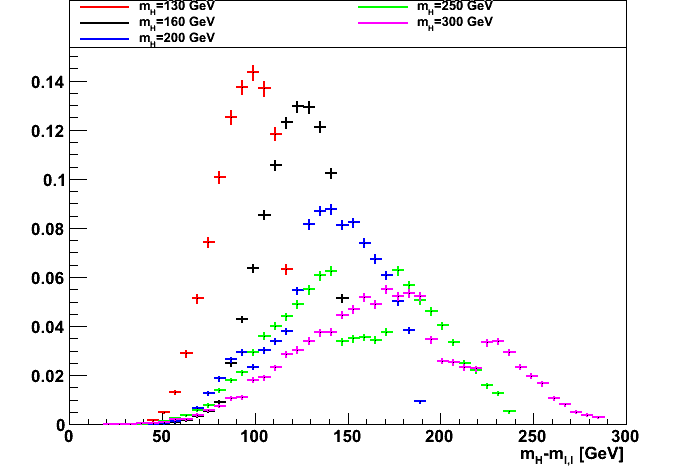
\includegraphics[width=.45\textwidth]{figures/higgsMllCutoff.png}
\caption{Difference between generated Higgs mass and di-lepton reconstructed invariant mass after WW cuts.}
\label{fig:higgsMllCutoff}
\end{figure}

\subsubsection{Estimation in Low Mass Range}

For low Higgs boson mass values ($m_{\rm{H}} \leq 200~\GeVcc$) events with $m_{\ell\ell} > 100~\GeVcc$ are used
to define a control region where the Higgs contribution is $<3\%$.

The procedure is as follows:
\begin{itemize}
\item the yield in the control region is measured after the lepton and jet selections 
(i.e. full selection except $m_{l,l}$, $m_T$ and $\Delta\phi_{ll}$ cuts) so that most of the systematics uncertainties 
cancel out (e.g. jet veto, lepton and trigger efficiencies); 
\item the contamination from other backgrounds (mainly $t\bar t$ and $W$+jets, for a total of $\sim$ 20\%) 
is subtracted using the corresponding data-driven techniques;
\item the obtained yield is scaled to the signal region using the control-to-signal region ratio from MC;
\item finally, the MC efficiency for $m_T$ and $\Delta\phi_{ll}$ cut is accounted to obtain the $WW$ contribution in the 
signal region after all cuts.
\end{itemize}

In order to consider this procedure as reliable we verify that 
the control-to-signal region ratio $R_{C/S}$ is stable using different generators (Table~\ref{tab:wwEstimationMC}) and 
we check that the efficiency of the $m_T$ and $\Delta\phi_{ll}$ cuts in the control region in data and MC is 
consistent (to be done).

\begin{table}[!htbp]
\begin{center}
\begin{tabular}{|c|c|c|} \hline
quantity                           &               MadGraph &                PYTHIA  \\ \hline
$R_{C/S}$                        &      0.205 $\pm$ 0.003 &      0.189 $\pm$ 0.007 \\
$\epsilon_{m_T}$(mass region)       &      0.874 $\pm$ 0.017 &      0.876 $\pm$ 0.046 \\
$\epsilon_{\Delta\phi}$(mass region) &      0.661 $\pm$ 0.015 &      0.655 $\pm$ 0.039 \\
$\epsilon_{m_T}$(side band)         &      0.391 $\pm$ 0.005 &      0.390 $\pm$ 0.011 \\
$\epsilon_{\Delta\phi}$(side band)   &      0.063 $\pm$ 0.003 &      0.046 $\pm$ 0.005 \\ \hline
\end{tabular}
\caption{Control-to-signal region ratio and cut efficiencies using MadGraph $qq\rightarrow WW$ and PYTHIA $gg\rightarrow WW$
vs PYTHIA inclusive $WW$. Results for $m_H=160~\GeVcc$ analysis in the 0-jet bin. 
Uncertainties are statistical and account for the MC sample luminosity. }
\label{tab:wwEstimationMC}
\end{center}
\end{table}

As a closure test, we apply the above procedure on simulated data, using MadGraph $qq\rightarrow WW$ and PYTHIA $gg\rightarrow WW$
as data and PYTHIA inclusive $WW$ as MC (errors are statistical only and are computed for a luminosity of $1~fb^{-1}$). 
For the moment we consider only the main contamination source in the side band region, top background; 
the expected yield for $1~fb^{-1}$ is 184.0 events (163.4 for $WW$ and 20.6 for $t\bar t$ plus $tW$).
The top contribution is evaluated by measuring the top tagging efficiency in a top-enriched sample (see dedicated section),
with a result of 15.6$\pm$5.2. 
Therefore, we estimate 168.4$\pm$14.5 $WW$ events in the side band region and, after applying
the control-to-signal region ratio and the cut efficiencies, 18.3$\pm$2.1 events in the $m_H=160~\GeVcc$ signal region 
(consistent with the expected value of 19.3$\pm$4.4).

The results for all considered Higgs masses are reported in Table~\ref{tab:wwEstimationRes0j}.

I AM NOT 100\% SYNCRONIZED YET!!!!

\begin{table}[!htbp]
\begin{center}
\begin{tabular}{|c|c|c|} \hline
$m_H~[\GeVcc]$ & WW estimation ($1~fb^{-1}$) & WW expected ($1~fb^{-1}$)  \\ \hline
120 & 43.3 $\pm$ 4.2 & 45.7 $\pm$ 6.8 \\
130 & 47.1 $\pm$ 4.5 & 49.5 $\pm$ 7.0 \\
140 & 42.7 $\pm$ 4.2 & 44.4 $\pm$ 6.7 \\
150 & 28.1 $\pm$ 3.1 & 28.9 $\pm$ 5.4 \\
160 & 18.3 $\pm$ 2.1 & 19.3 $\pm$ 4.4 \\
200 & 11.6 $\pm$ 1.3 & 12.3 $\pm$ 3.5 \\
 \hline
\end{tabular}
\caption{Result of $WW$ estimation for different Higgs mass analyses in the 0-jet bin. }
\label{tab:wwEstimationRes0j}
\end{center}
\end{table}


%Systematics are evaluated repeating the procedure varying the usual suspects.

%
%\subsection{Estimation in high mass range}
%We take it from MC.



%The nonresonant $qq \to \WW$ contribution in the $\hww$ signal region is 
%estimated from data using the dilepton mass distribution. For a given Higgs 
%boson mass, the region with a small contribution from Higgs boson decays is 
%selected and simulation is used to extrapolate this background into the signal 
%region. For low Higgs boson mass values ($m_{\rm{H}} < 200~\GeVcc$) events 
%with $m_{\ell\ell} > 100~\GeVcc$ are used, while for $m_{\rm{H}} > 200~\GeVcc$ 
%events with $m_{\ell\ell} < 100~\GeVcc$ are used. The statistical uncertainty 
%on the estimate of the nonresonant $\WW$ background with the current data 
%sample is approximately 50\%. For the 1- and 2- jet bin cases we use the results
%from the 0-jet bin, and then extrapolate to each jet bin.
%
%The $gg \to \WW$ background contribution has to be taken from simulated events 
%since we do not have enough sensitivity in the data to measure it. We assign a 
%50\% uncertainty to the overall normalization~\cite{ggWWError}. This is 
%obtained by studying the change in the cross-section when varying the parton 
%distribution functions (PDFs), QCD renormalization and scales.
